{\em Auteur: Laura Vranken}\\

\noindent
De Drone Autopilot zorgt voor de besturing van de drone. Hij bepaalt zijn positie relatief ten opzichte van zijn doel a.d.h.v. twee beelden, gegeneerd door de dronecamera's. Bovendien kunnen ze opgevraagd worden vanuit de \textit{GUI} van het Virtual Testbed. Vervolgens zorgt de Autopilot ervoor dat de drone juist geori\"enteerd staat en naar zijn doel toe vliegt. Wanneer de drone zijn doel (in deze eerste fase is dit een rode bol) bereikt, moet hij daarin blijven zweven. Tenslotte moet de Autopilot ook rekening houden met een mogelijke invloed van wind die de drone van zijn koers doet afwijken.
\\
\\
Ten eerste moeten de beelden die de Autopilot van de Virtual Testbed binnenkrijgt, geanalyseerd worden. Dit gebeurt door iteratief de integer waarden van elke pixel te vergelijken met de waarde van de kleur rood. Alle rode pixels worden bijgehouden door hun positie ten opzichte van het beeld, uitgedrukt in rij en kolom, op te slaan. We baseren onze komende berekeningen op het midden van de bol. Dat midden kan bepaald worden door het zwaartepunt van de rode pixels te berekenen via het gemiddelde van de opgeslagen co\"ordinaten.
\\
Indien de Autopilot geen rode pixels detecteert, zal de drone 360 graden ronddraaien of m.a.w. een yaw beweging uitvoeren, totdat in beide beelden rode pixels verschijnen. Dan zal de Autopilot stoppen met draaien en zijn positie tegenover het doel berekenen.
\\
\\
Om zijn positie tegenover het doel te berekenen, bepalen we eerst de diepte. Dit kan met behulp van de formule van stereo vision \cite{website:techbriefs} uitgewerkt worden. Zie figuur \ref{fig:DiepteberekeningDroneEnDoel} voor een grafische weergave van de berekening.
\begin{figure}[h]
	\centering
	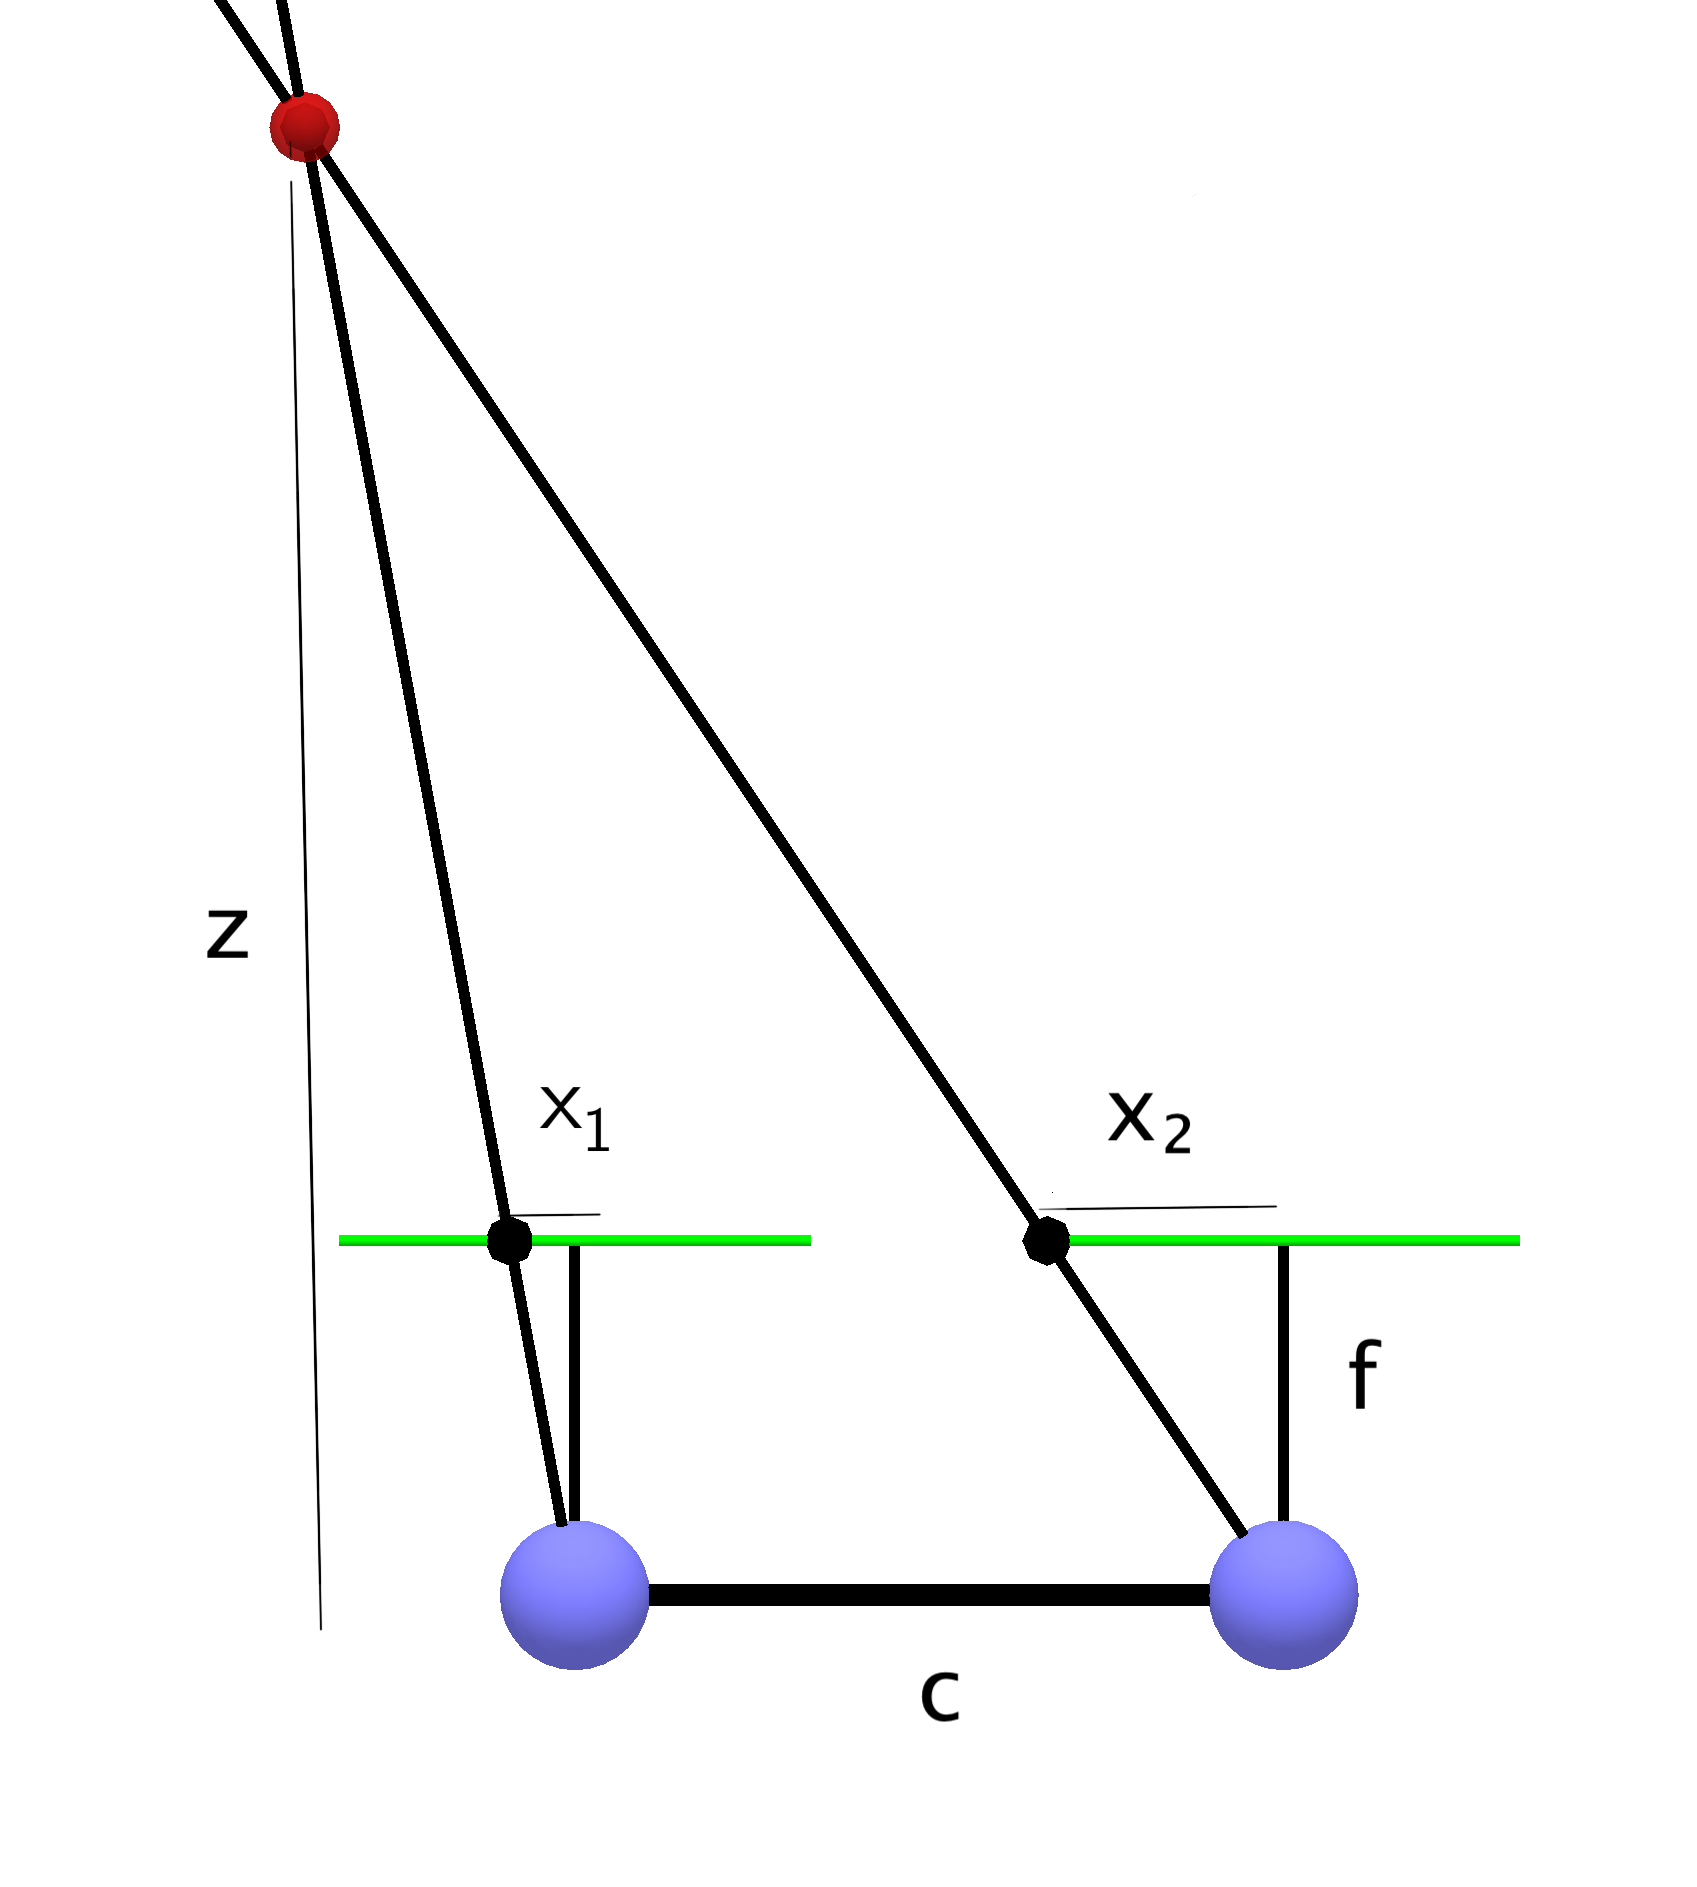
\includegraphics[width=0.3\textwidth]{DiepteberekeningDroneEnDoel.png}
	\caption{Diepteberekening tussen drone en doel. In formulevorm: \(z = \frac{c * f}{x_1 - x_2}\).}
	\label{fig:DiepteberekeningDroneEnDoel}
\end{figure}
\\
Vervolgens bepalen we de hoek waaronder de drone een yaw beweging moet uitvoeren om recht naar het doel gericht te zijn. Deze formule wordt afgeleid via de goniometrische regels. Zie figuur \ref{fig:RelatieveHorizontaleHoek} voor grafische ondersteuning. 

Berekening brandpuntsafstand f:
\begin{equation} \label{eq:RelatieveVerticaleHoekBegin}
\tan(\frac{\delta}{2}) = \frac{\frac{b}{2}}{f}
\end{equation}
\begin{equation} 
f = \frac{\frac{b}{2}}{\tan(\frac{\delta}{2})}
\end{equation}
Berekening afstand x:
\begin{equation} 
\frac{x_2}{f} = \frac{x}{z}
\end{equation}
\begin{equation} \label{eq:RelatieveVerticaleHoekEind}
x = z * \frac{x_2}{f}	
\end{equation}
\\
\\
Om tenslotte naar het doel te kunnen vliegen, moet een evenwicht gevonden worden tussen pitch en thrust. De pitch hoek wordt gekozen zodat het zwaartepunt van het doel nog juist in beeld blijft. Die hoek is gelijk aan de helft van de verticale hoek die het beeld overspant min de verticale hoek waaronder de bol zich tegenover de drone bevindt, zie figuur \ref{fig:RelatieveVerticaleHoek}. 
\\
\begin{figure}
	\centering
	\begin{minipage}{.45\textwidth}
		\centering
		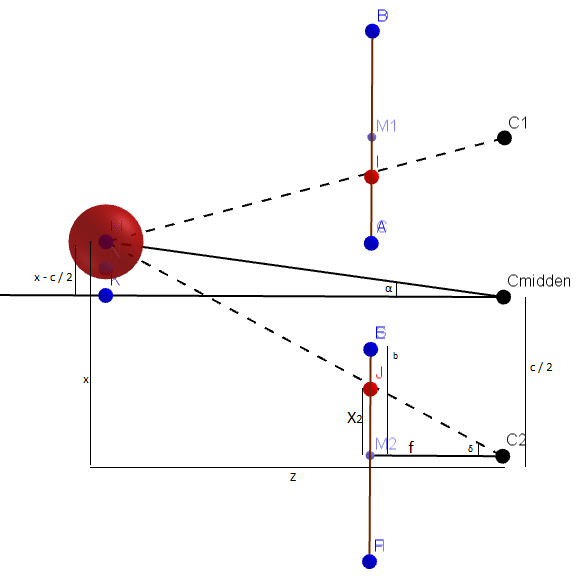
\includegraphics[width=0.8\textwidth]{RelatieveHorizontaleHoek.png}
		\caption{Relatieve horizontale hoek.}
		\label{fig:RelatieveHorizontaleHoek}
	\end{minipage}
	\begin{minipage}{.45\textwidth}
		\centering
		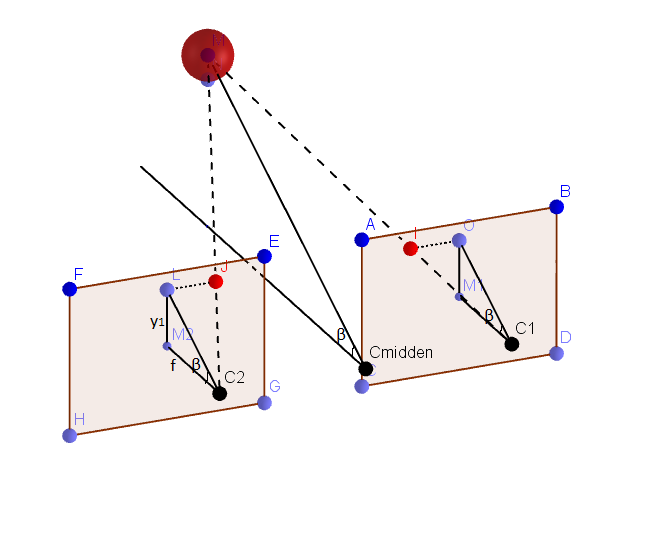
\includegraphics[width=0.96\textwidth]{RelatieveVerticaleHoek.png}
		\caption{Relatieve verticale hoek.}
		\label{fig:RelatieveVerticaleHoek}
	\end{minipage}%
	\caption*{Links wordt de relatieve horizontale hoek tussen drone en doel weergegeven door \(\tan(\alpha) = \frac{x-\frac{c}{2}}{z}\), voor de volledige uitwerking zie formule \ref{eq:RelatieveVerticaleHoekBegin} tot \ref{eq:RelatieveVerticaleHoekEind}.\\
		Rechts wordt de relatieve verticale hoek weergegeven tussen drone en doel. De relatie wordt gegeven door volgende formule: \(\tan(\beta) = \frac{y_1}{f}\).}
\end{figure}
\\
Wanneer de pitch hoek vastligt, kan de hoeveelheid thrust berekend worden zodat de drone in rechte lijn naar het doel kan vliegen. Voor een gedetaileerde uitwerking zie \ref{sec:AlgoritmesAutopilot}.
\\
\\
Tenslotte moet dit proces herhaaldelijk worden uitgevoerd ten gevolge van de invloed van wind. De wind kan de drone namelijk uit koers brengen. Hierdoor zal de drone telkens zijn positie moeten herberekenen en zich opnieuw moeten herori\"enteren. Ook kan de wind ervoor zorgen dat de drone een roll uitvoert. Deze moet eerst gecompenseerd worden, vooraleer we verder onze berekeningen kunnen uitvoeren.
\\
De drone bereikt zijn doel wanneer de Autopilot niks anders dan rode pixels opvangt. De drone zal dan de opdracht krijgen om zijn pitch te compenseren en vervolgens enkel via thrust de zwaartekracht tegen te werken.
\\
Het effectief laten vliegen van de drone gebeurt in de Virtual Testbed waar de motoren worden aangestuurd. De Autopilot zendt enkel de verhouding in graden per seconden door waaronder pitch, yaw en roll moeten worden uitgevoerd en thrust in Newton. Het is slechts door herhaaldelijk te controleren hoe ver nog gedraaid moet worden, dat kan besloten worden wanneer de beweging volledig uitgevoerd is en wanneer er gestopt mag worden.